\section{Multitasking experiments on NV}

The multitasking evaluation was done in two parts:
%
\begin{itemize}
    \item \textbf{Quantum tomography while multitasking}: Executing a single \ac{DQC} application (on client and server) and a single \ac{LGT} application (on client only) where it was verified that the \ac{LGT} application produces expected quantum results (see~\cref{qnodeos:sec:multitasking-tomography}).
    \item \textbf{Scaling the number of applications}: Executing $N$ \ac{DQC} applications and $N$ \ac{LGT} applications, where the classical device utilization metric was compared with a version of \ac{QNodeOS} without multitasking, and where we investigated the behavior of the \ac{QNPU} scheduler on the client in the context of multiple programs (see~\cref{qnodeos:sec:multitasking-scaling}).
\end{itemize}
%
The network schedule was set as in the previous \ac{DQC} experiment for direct comparison.

\subsection{Mocked entanglement}
\label{qnodeos:sec:mocked_entanglement}

For the multitasking evaluation, we focused on the behavior of \ac{QNodeOS}, and opted not to use the standard entanglement generation procedure in our \ac{NV} \acp{QDevice} as done in the \ac{DQC} experiments (\cref{qnodeos:sec:delcomp}) to allow for a simpler experiment. Instead, we used a mocked entanglement generation process on the \acp{QDevice} (executing entanglement actions without entanglement): Weak-coherent pulses on resonance with the \ac{NV} transitions, that follow the regular optical path, are employed to trigger the \ac{CPLD} in the entanglement heralding time-window.

We stress that in our multitasking experiments, the exact same physical instructions are sent to the \ac{QDevice} as would be done when using real entanglement, and the exact same responses are sent back. Therefore, \ac{QNodeOS} needed to perform the same operations (including scheduling decisions) as it would have needed to do with real entanglement. Furthermore, we aimed to keep the rate of entanglement `success' in the \acp{QDevice} the same order of magnitude as that of the \ac{DQC} experiments (10.14\,\acp{EPR}/s compared to 2.37\,\acp{EPR}/s in the \ac{DQC} experiment) by keeping the mean-photon number of the weak-coherent pulse comparable to $p_C$ and $p_S$ (in the order of $\sim10^{-4}$). 

\subsection{Tomography results}
\label{qnodeos:sec:multitasking-tomography}

We perform tomography when not multi-tasking, in order to verify our expectation that multi-tasking should not affect the quantum performance of \ac{LGT}: The tomography results of the \ac{LGT} application in the multitasking scenario are given in \cref{qnodeos:fig:fig4}c. We also ran the same \ac{LGT} application on the client in a non-multitasking scenario. In this case, the client ran the \ac{LGT} application and there was no \ac{DQC} application run at all (the server did nothing). The tomography results of \ac{LGT} for the non-multitasking scenario are given in \cref{qnodeos:fig:tomography-no-multitasking}. The results are slightly different since the multitasking experiment was done on a different day than the non-multitasking experiment. However, within error bars we verify that multitasking does not affect the quantum performance of the \ac{LGT} application.

\begin{figure}
\centering
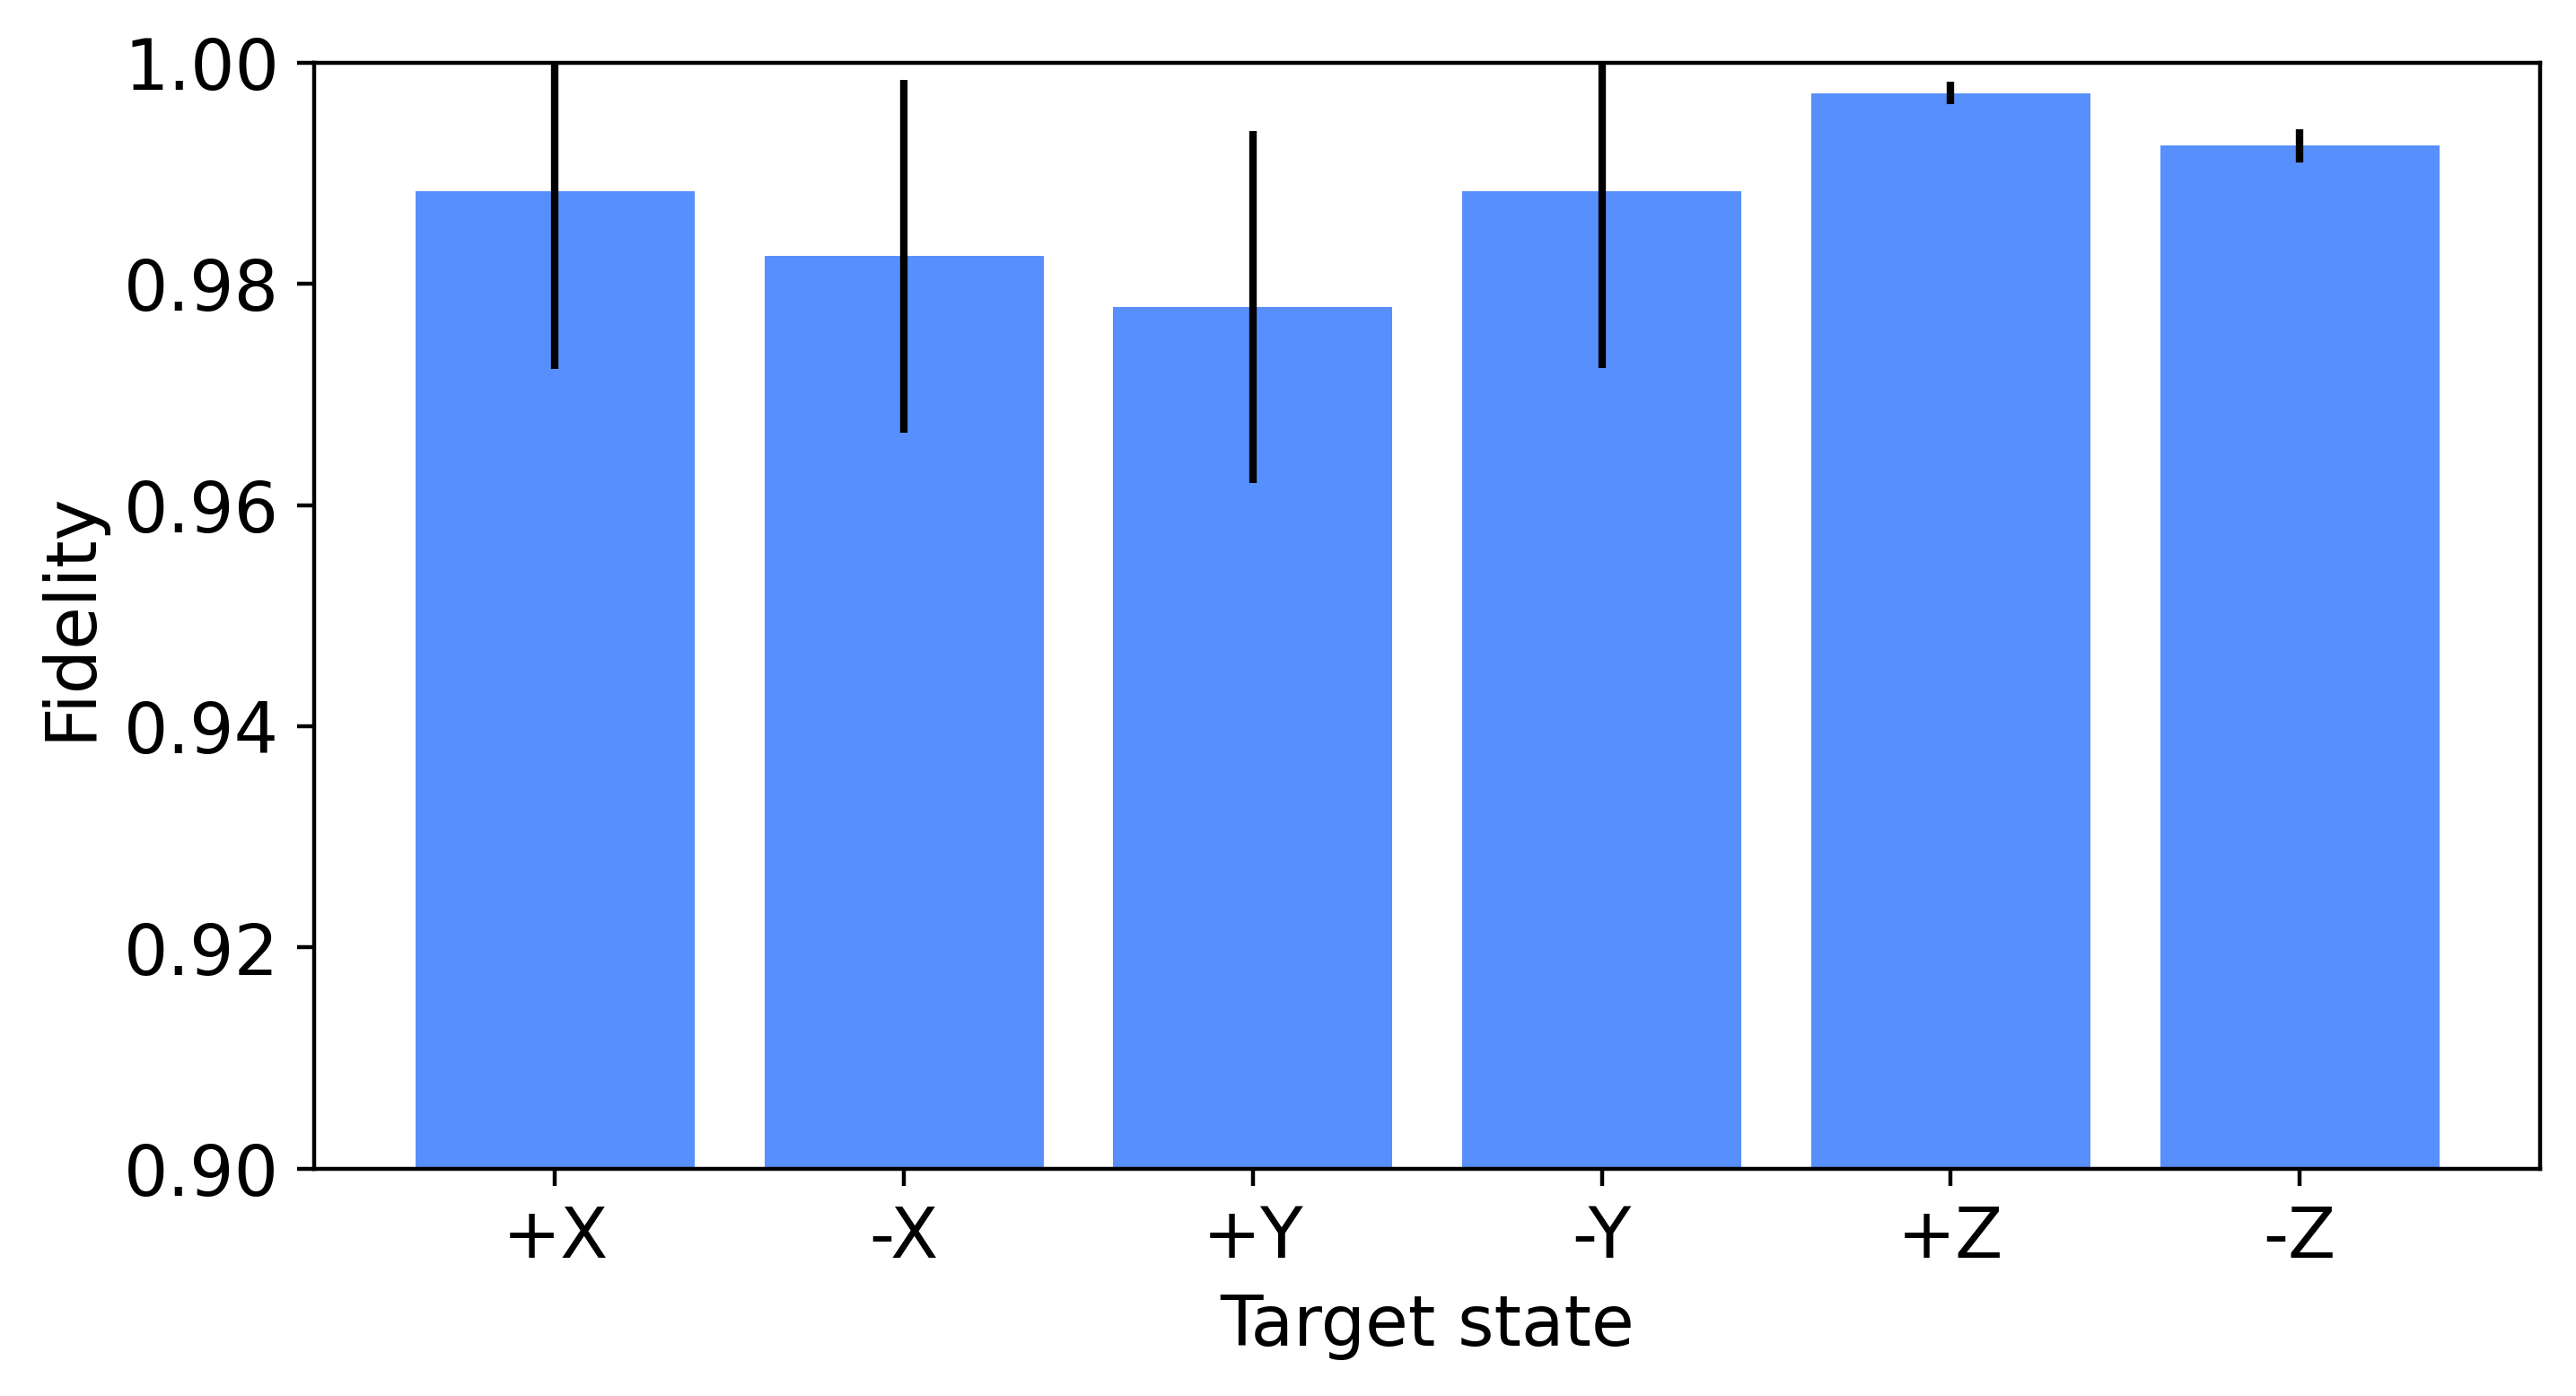
\includegraphics[width=\linewidth]{figures/qnodeos/supplementary/plots/noMT_gate_tomography.png}
\caption{Local Gate Tomography results on the client node in a non-multitasking scenario.}
\label{qnodeos:fig:tomography-no-multitasking}
\end{figure}

\subsection{Scaling to more than two applications}
\label{qnodeos:sec:multitasking-scaling}

\subsubsection{QNPU processes and steps}

For the scaling evaluation, we did an experiment for each $N \in \{1, 2, 3, 4, 5\}$. For each experiment, the client \ac{CNPU} started $N$ \ac{DQC}-client programs and $N$ \ac{LGT} programs concurrently (pseudocode in \cref{src:cnpu_runner}), and the server \ac{CNPU} started $N$ \ac{DQC}-server programs. In this section we discuss the observed behavior of the client and server \acp{QNPU} during these experiments. The client \ac{QNPU} has $2N$ user processes ($N$ \ac{DQC} user processes and $N$ LGT user processes), each of which continuously receives quantum blocks in the form of \ac{NetQASM} subroutines (C1 for \ac{DQC} processes and L1 for \ac{LGT} processes). These $2N$ user processes and the single client network process are scheduled by the client \ac{QNPU} scheduler. The server has $N$ user processes (all for \ac{DQC}) which are scheduled together with the server network process by the server \ac{QNPU} scheduler. \cref{qnodeos:fig:multitasking-default} shows a schematic diagram of the nominal (most often occurring) pattern of scheduling.

In both S1 and C1, there is a single \texttt{create\_epr} \ac{NetQASM} instruction~\cite{dahlberg_2022_netqasm} for creating entanglement with the other node, followed by a \texttt{wait\_all} \ac{NetQASM} instruction that waits until the request entangled qubit is delivered. The \texttt{create\_epr} instruction is handled by the \ac{QNPU} processor by sending the entanglement request to the network stack. Upon executing the \texttt{wait\_all} instruction, the user process executing this subroutine (S1 or C1) goes into the waiting state (green stop sign in \cref{qnodeos:fig:multitasking-default}). When the network process completes (having created the entangled qubit), the user process can be resumed, finishing the subroutine (C1 or S1). 

On the server \ac{QNPU}, for each \ac{DQC} user process $U$ the following sequence is repeated:
%
\begin{itemize}
    \item $U$ is in the \textit{idle} state;
    \item \ac{NetQASM} subroutine S1 is submitted by the \ac{CNPU} to the \ac{QNPU}, moving $U$ to \textit{ready};
    \item $U$ is activated; S1 is executed until it hits the \texttt{wait\_all} instruction; $U$ goes into the \textit{waiting} state;
    \item The network process handles the entanglement request for S1 until \ac{EPR} creation succeeds; $U$ goes into \textit{ready} again;
    \item $U$ is activated; S1 is executed until completion; $U$ goes to \textit{idle};
    \item \ac{NetQASM} subroutine S2 is submitted by the \ac{CNPU}; $U$ goes to \textit{ready};
    \item $U$ is activated; S2 is executed until completion; $U$ goes to \textit{idle}.
\end{itemize}
%
The above sequence is for one execution of the \ac{DQC} circuit (\cref{qnodeos:fig:fig3}a), and is hence repeated many times.

On the client \ac{QNPU}, for each \ac{DQC} user process $U$ the following sequence is repeated:
%
\begin{itemize}
    \item $U$ is in the \textit{idle} state;
    \item \ac{NetQASM} subroutine C1 is submitted by the \ac{CNPU}, moving $U$ to \textit{ready};
    \item $U$ is activated; C1 is executed until it hits the \texttt{wait\_all} instruction; $U$ goes into the \textit{waiting} state;
    \item the network process handles the entanglement request for C1 until \ac{EPR} creation succeeds; $U$ goes into \textit{ready} again;
    \item $U$ is activated; C1 is executed until completion; $U$ goes to \textit{idle}.
\end{itemize}
%
The above sequence is for one execution of the \ac{DQC} circuit (\cref{qnodeos:fig:fig3}a), and is hence repeated many times.

On the client \ac{QNPU}, for each \ac{LGT} user process $U$ the following sequence is repeated:
%
\begin{itemize}
    \item $U$ is in the \textit{idle} state;
    \item \ac{NetQASM} subroutine L1 is submitted by the \ac{CNPU}, moving $U$ to \textit{ready};
    \item $U$ is activated; L1 is executed until completion; $U$ goes to \textit{idle}.
\end{itemize}
%
The above sequence is for one execution of the \ac{LGT} circuit (\cref{qnodeos:fig:fig4}a), and is hence repeated many times.

For the above sequences for user processes, only the internal order is fixed; the time in between steps depends on the \ac{QNPU} scheduler, as well as the time at which the \ac{CNPU} submits subroutines. Furthermore, since there are multiple user processes at the same time (for the server, only for $N > 1$), the above steps happen for each user process $U_i$ and the steps are interleaved. \cref{qnodeos:fig:multitasking-default,qnodeos:fig:multitasking-2-apps,qnodeos:fig:multitasking-wait-on-client} show examples of how these user processes can be interleaved on both client and server \ac{QNPU}.

\subsubsection{DQC and LGT interleaving}

We investigate the degree of interleaving the execution of \ac{DQC} and \ac{LGT}, in particular how many \ac{LGT} subroutines are executed when a \ac{DQC} process is waiting: The client \ac{QNPU} executes both \ac{DQC} and \ac{LGT} user processes. \ac{DQC} user processes are often in the waiting state. This happens when their C1 subroutine is suspended, waiting for the network process to handle their entanglement request. The network process is only activated at the beginning of a time bin, which happens only every 10\,ms, or when a user process finishes executing a subroutine, the latter not occurring very frequently for low number of programs $N$. Furthermore, \ac{DQC} user processes can be in the idle state, namely when they completed execution of C1 for some iteration $i$ of the \ac{DQC} circuit, but are still waiting for the \ac{CNPU} to send C1 for iteration $i+1$. In both these types of `gaps` (waiting or idle), \ac{LGT} subroutines can be executed (each taking $\approx$2.4\,ms). \cref{tab:multitasking_numbers} lists the maximum number of consecutive \ac{LGT} subroutines that were executed in between \ac{DQC} subroutines  for both types of gaps. 

\subsubsection{Subroutine (Quantum block) execution order}

We investigate whether the \ac{QNPU} schedules quantum subroutines in a different order than they arrived from the \ac{CNPU}. As expected, we find that this is the case. Although the \ac{QNPU} handles subroutines from the \ac{CNPU} first-come-first-served, some of these subroutines (in our experiments, precisely the \ac{DQC} subroutines that wait for entanglement) are put into the waiting state. This allows the \ac{QNPU} to schedule other subroutines (in our experiments, we observe \ac{LGT} subroutines being executed), even if they arrived later from the \ac{CNPU} than the waiting \ac{DQC} subroutine. Schematic overviews of such scheduling that we observed are depicted in \cref{qnodeos:sec:multitasking_patterns}.

\subsubsection{User process idle times}

We examine the number of times, and the duration, that a user process is idle waiting for submission of a subroutine from the \ac{CNPU} as a function of $N$: A user process is \textit{idle} when there are currently no subroutines associated with the process pending to be executed. This means that the \ac{QNPU} waits, at least for this user process, until the \ac{CNPU} sends the next subroutine for the user process. \cref{tab:multitasking_numbers} lists the number of times and durations of moments at which all client \ac{QNPU} user processes are idle. This number and their durations decrease for larger values of $N$. This is expected since there are more active processes, and hence more subroutines being sent from the \ac{CNPU} for different processes. In most cases, when finishing a subroutine for user process $U$, there is then another user process $U'$ already waiting with another subroutine to execute.

\subsubsection{Network process start delays}

We examine the scheduling behavior of the network process in relation to user processes. We expect that due to the fact we use a non-preemptive scheduler, a network process may not be activated at the start of a network time bin, due to a user process still being executed. We investigate the occurrence of such events in our multi-tasking experiment, including the delay with which the network process is started in such a scenario (see \cref{tab:multitasking_numbers}): When a user process submits and entanglement request to the network stack, this request is handled at the earliest when the network process is activated. This happens either at the start of the next network time bin, or when a user process finishes a subroutine. Therefore, there is often some time in between submitting the request and the network process handling it. This waiting time is in most cases bounded by 10\,ms, since that is the length of a time bin, and all time bins are assigned to networking in our experiment. However, in some cases the client may still be executing a \ac{LGT} subroutine when a new time bin starts, delaying the start of the network process until this subroutine has finished. We expect however that in all cases, as soon as such an \ac{LGT} subroutine finishes, the \ac{QNPU} scheduler then immediately schedules the network process, and not another \ac{LGT} subroutine. We found that the maximum difference between time bin start and network process start is 2.59\,ms, which verifies that indeed at most one \ac{LGT} subroutine is sometimes executed during a time bin start (\ac{LGT} subroutine execution duration being $\approx$2.4\,ms.)

We remark that with increasing $N$, the network process is delayed more frequently by a \ac{LGT} subroutine. This is expected due to the fact more subroutines from different user processes await execution. Consequently, with increasing $N$ it also happens more frequently that the client and server do not start execution of the network process in the same time-bin (see below).

\subsubsection{Client waits for server and vice versa}

In order to better understand the concurrent execution of multiple applications (here \ac{DQC} and \ac{LGT}) and corresponding programs, we investigate scenarios and times in which the client waits for the server (or vice versa). 

The client and server open an \ac{ER} socket at the beginning of each \ac{DQC} application. So, during runtime, there are $N$ \ac{ER} sockets opened on the server \ac{QNPU} (one for each \ac{DQC} process) and $N$ \ac{ER} sockets opened on the client \ac{QNPU} (one for each \ac{DQC} process). In each \ac{DQC} application, the client \ac{QNPU} user process for that \ac{DQC} application is the `initiator' (see \cref{qnodeos:sec:design_er_socket}). This means that as soon as the client user process submits a request for entanglement (from within C1), both server and client \ac{QNPU} start their network process to handle it (at the start of the next time bin, and provided the network process should not first handle a request from a user process from another \ac{DQC} application).

It can happen that the client \ac{QNPU} and server \ac{QNPU} do not start their network process at the same time bin. This mostly happens when one of the nodes is still busy executing a user process subroutine when a time bin starts, as explained above. If this happens, the \ac{QNPU} that did already start their network process sends entanglement instructions to their \ac{QDevice}, but this will not result in physical entanglement attempts since the other \ac{QDevice} is not available (leading to a entanglement sync failure, see \cref{qnodeos:sec:qdevice-sync}). \cref{tab:multitasking_numbers} lists the number of times that this happened.

For each of the $N$ \ac{DQC} applications that are running on client and server, and for each execution of the \ac{DQC} circuit in those applications, there is a single entanglement request from the client (in C1) and a single entanglement request from the server (in S1). For each of these request pairs, the client at some point starts the network process and handles this request, and the server at some point starts the network process and handles its corresponding request. For each such pair of requests, the following scenarios can happen:
%
\begin{enumerate}
    \item Client and server \ac{QNPU} start their network process in the same time-bin (one of them may start a bit later than the start of the time-bin because it needs to complete a quantum subroutine).
    \item The client starts its network process in time-bin $k$ but the server starts it at some time-bin $>k$. This happens when the server still has a qubit in memory when time-bin $k$ starts. Therefore, the server cannot activate its network process yet. A qubit still being in memory happens when the server \ac{QNPU} has executed S1 for some \ac{DQC} process (which produced an entangled qubit) but has not yet executed S2 (in which the qubit is measured and hence freed).
    \item The server starts its network process in time-bin $k$ but the client starts it at time-bin $k+1$. This happens (although rarely) when the client user process puts the entanglement request to the network stack just before the start of $k$. The server will immediately start attempts at $k$, but the client itself is still processing and `misses' $k$; the client then only starts at time-bin $k+1$.
\end{enumerate}

\cref{tab:multitasking_numbers} lists how often the above scenarios happen for each $N$.

\begin{table*}
    \centering
    \begin{tabular}{|r|c|c|c|c|c|}
    \hline
    \textbf{Parameter} & \textbf{N = 1} & \textbf{N = 2} & \textbf{N = 3} & \textbf{N = 4} & \textbf{N = 5} \\ 
    \hline
    average no. \ac{LGT} subroutines in between any \ac{DQC} subroutines & 0.83 & 1.42 & 1.59 & 1.65 & 1.65 \\
    max no. consecutive \ac{LGT} subroutines in between \ac{DQC} subroutines & 3 & 4 & 6 & 7 & 8 \\
    max no. consecutive \ac{LGT} subroutines when a \ac{DQC} is in waiting state & 2 & 3 & 4 & 4 & 4 \\
    \% of times that $\geq 1$ \ac{LGT} subroutines fills time waiting for time bin  & 56 & 81 & 99 & 99 & 100 \\
    no. times that network process is delayed by a \ac{LGT} subroutine & 88/360 & 212/720 & 554/1080 & 940/1440 & 1170/1800 \\
    no. time windows in which all user processes are idle & 399 & 56 & 4 & 1 & 0 \\
    Average length of idle time window (ms) & 10 & 5.9 & 5.9 & 8.3 & --- \\
    Maximum length of idle time window (ms) & 152 & 31 & 15 & 8.3 & --- \\
    \% client and server start network process at same time bin & 95.8 & 58.2 & 42.1 & 42.4 & 38.5 \\
    \% server started network process 1 time bin after client & 0.8 & 37.9 & 50.1 & 50.9 & 53.1 \\
    % \% server started network process 2 time-bins after client & 0.0 & 3.2 & 5.6 & 4.9 & 6.6 \\
    % \% server started network process $>2$ time-bins after client & 0.0 & 0.1 & 2.1 & 1.7 & 1.9 \\
    \% server started network process $> 1$ time bins after client & 0.0 & 3.3 & 7.7 & 6.6 & 8.4 \\
    \% client started network process 1 time bin after server & 3.3 & 0.6 & 0.1 & 0.1 & 0.0 \\
    \hline
    \end{tabular}
    \caption{Overview of values derived from the multitasking experiments in which $N$ \ac{DQC} applications (on client and server) and $N$ \ac{LGT} applications (client only) were executed concurrently, for $N \in \{1, 2, 3, 4, 5\}$.}
    \label{tab:multitasking_numbers}
\end{table*}


